%PDF DI RIFERIMENTO: 06_System Design.pdf + DesignPractices.pdf, 08_Architetture Software.pdf, 08_Architetture.pdf

\chapter{Object Design}
    La progettazione orientata agli oggetti è la fase di sviluppo del software nella quale si definisce il dettaglio implementativo dei vari sottosistemi. \\
    Tali sottosistemi devono soddisfare i requisiti identificati, e sono costruiti sulla base degli oggetti individuati nel dominio del problema, ai quali inevitabilmente saranno aggiunti nuovi oggetti per giungere alla soluzione del problema. \\
    Avendo impiegato un approccio "orientato ai casi d'uso", all'interno del sistema, vi sono tanti \textbf{sottosistemi} quanti sono gli use case, ognuno dei quali si occupa di uno e uno solo use case. \\
    Ogni sottosistema è organizzato in quattro macrosezioni:
    
    \begin{itemize}
        \item (Client) Lo strato di presentazione dell'interfaccia utente;
        \item (Client) Lo strato di controllo dell'interfaccia utente che costruisce l'interfaccia, controlla la validità dei dati inseriti, gestisce le richieste da inviare al server attraverso le REST API, gestisce le risposte ricevute dal server attraverso le REST API;
        \item (Server) Lo strato di controllo dei dati che controlla la validità dei dati in arrivo, invia i dati da archiviare allo strato di archiviazione, gestisce le risposte da inviare al client attraverso le REST API, gestisce le richieste ricevute dal client attraverso le REST API;
        \item (Server) Lo strato di archiviazione dei dati che si occupa di comunicare con la base di dati per il recupero e il salvataggio dei dati.
    \end{itemize}

    \clearpage

    \section{Design Pattern}
        \subsection{Client}

        \subsection{Resource Server}
            L'architettura adottata per il sottosistema \textbf{Resource Server} (da qui in avanti chiamato semplicemente \textbf{Server}) è un'architettura di tipo \textbf{esagonale}. L'obiettivo di tale architettura è di definire una \textbf{separazione netta} tra la business logic del dominio (anche detto \textit{domain layer}) e tutto ciò che sono i fattori esterni, ovvero il layer di interfaccia con l'utente (anche detto \textit{application layer}) e il layer di persistenza (anche detto \textit{infrastracture layer}), attraverso una serie di interfacce ben definite. \\
            L'obiettivo di tale scelta è quello di migliorare la manutenibilità, la scalabilità e la modularità del backend, definendo così interfacce ben definite che permettono a più team di sviluppo di lavorare parallelamente, conoscendo esattamente il contratto per le interazioni tra la logica del dominio e dei protocolli di comunicazione tra l'applicazione e i suoi adattatori. \cite{AppMaster1}
            
            In particolare, il design pattern adottato per il domain layer è di tipo \textbf{Domain Driven}. Un approccio di tipo Domain Driven permette di avere un'\textbf{alta coesione} e \textbf{ridurre al minimo l'accoppiamento} tra le classi della business logic, dando a ciascuna classe del domain layer un solo motivo per cambiare: un cambiamento nell'entità del dominio corrispondente.
            \begin{figure}[htbp!]
                \centering
                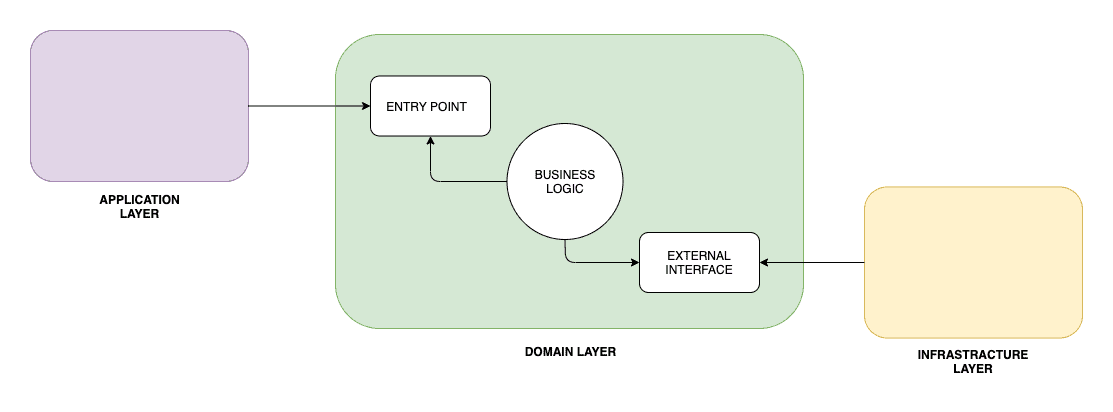
\includegraphics[width=1\linewidth]{Immagini/Object Design/DDD-Layers.jpg}
                \caption{Schema dell'architettura adottata (backend)}
                \cite{Baeldung1}
            \end{figure}

            In particolare, il backend è così organizzato:
            \begin{itemize}
                \item L'\textit{application layer} contiene le classi responsabili di esporre le REST API che verranno chiamate dall'utente. E' dipendente solo e unicamente da classi DTO, che si occupano di raccogliere le informazioni ricevute sottoforma di HTTP Request e saranno tradotte in HTTP Response. \cite{Baeldung2}
                \item Il \textit{domain layer} contiene le classi responsabili della business logic, che dipende solo e unicamente dalle classi del dominio, ovvero le entità. Al suo interno troviamo anche classi responsabili di tradurre i DTO in entità del dominio. \\
                Inoltre, grazie all'interfaccia offerta dalla \textbf{Java Persistance API}, le classi necessarie per la comunicazione con il persistance layer sono gestite da Spring Boot attraverso una Spring dependency.
                \item Il \textit{persistance layer} contiene i driver responsabili della comunicazione con il database.
            \end{itemize}

    \clearpage

    \section{Class Diagram}
        A seguito delle considerazioni fatte ai punti precedenti, in questa sezione verranno rappresentati i diagrammi delle classi di design del client e del server.
    
        \subsection{Client}
            % Class Diagram costruito con PlantUML
            \begin{figure}[htbp!]
                \includegraphics[width=0.9\linewidth]{Immagini/Diagrammi/Class Diagram/Design/ClassDiagramClient.pdf}
            \caption{Class Diagram client}
            \label{fig:Class Diagram client}
            \end{figure}
    
        \subsection{Server}
            % Class Diagram costruito con PlantUML
            \begin{figure}[htbp!]
                \includegraphics[width=0.35\linewidth]{Immagini/Diagrammi/Class Diagram/Design/ClassDiagramServer.pdf}
            \caption{Class Diagram server}
            \label{fig:Class Diagram server}
            \end{figure}

    \clearpage
    
    \section{Sequence Diagram}
        In questa sezione saranno rappresentati i diagrammi di sequenza di design del client e del server per i casi d'uso individuati nella fase di Requirement Analysis.
        
        \subsection{I caso d'uso: Crea un’asta inversa}
            \begin{figure}[htbp!]
                \centering
                    \includegraphics[width=0.47\linewidth]{Immagini/Diagrammi/Sequence Diagram/Design/Client Sequence Design/ClientSequenceCreaAstaDesign.pdf}
                \caption{Sequence Diagram di design creazione asta inversa (client)}
                \label{fig:Sequence Diagram di design creazione asta inversa (client)}
            \end{figure}

            \begin{figure}[htbp!]
                \centering
                    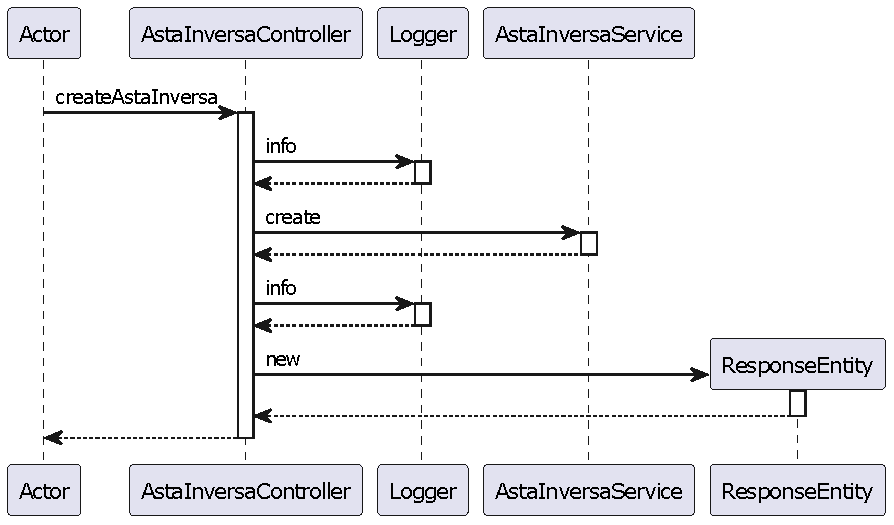
\includegraphics[width=1\linewidth]{Immagini/Diagrammi/Sequence Diagram/Design/Server Sequence Design/ServerSequenceCreaAstaDesign.pdf}
                \caption{Sequence Diagram di design creazione asta inversa (server)}
                \label{fig:Sequence Diagram di design creazione asta inversa (server)}
            \end{figure}

        \clearpage

        \subsection{II caso d'uso: Accetta un'offerta ricevuta all'asta silenziosa}
            \begin{figure}[htbp!]
                \centering
                    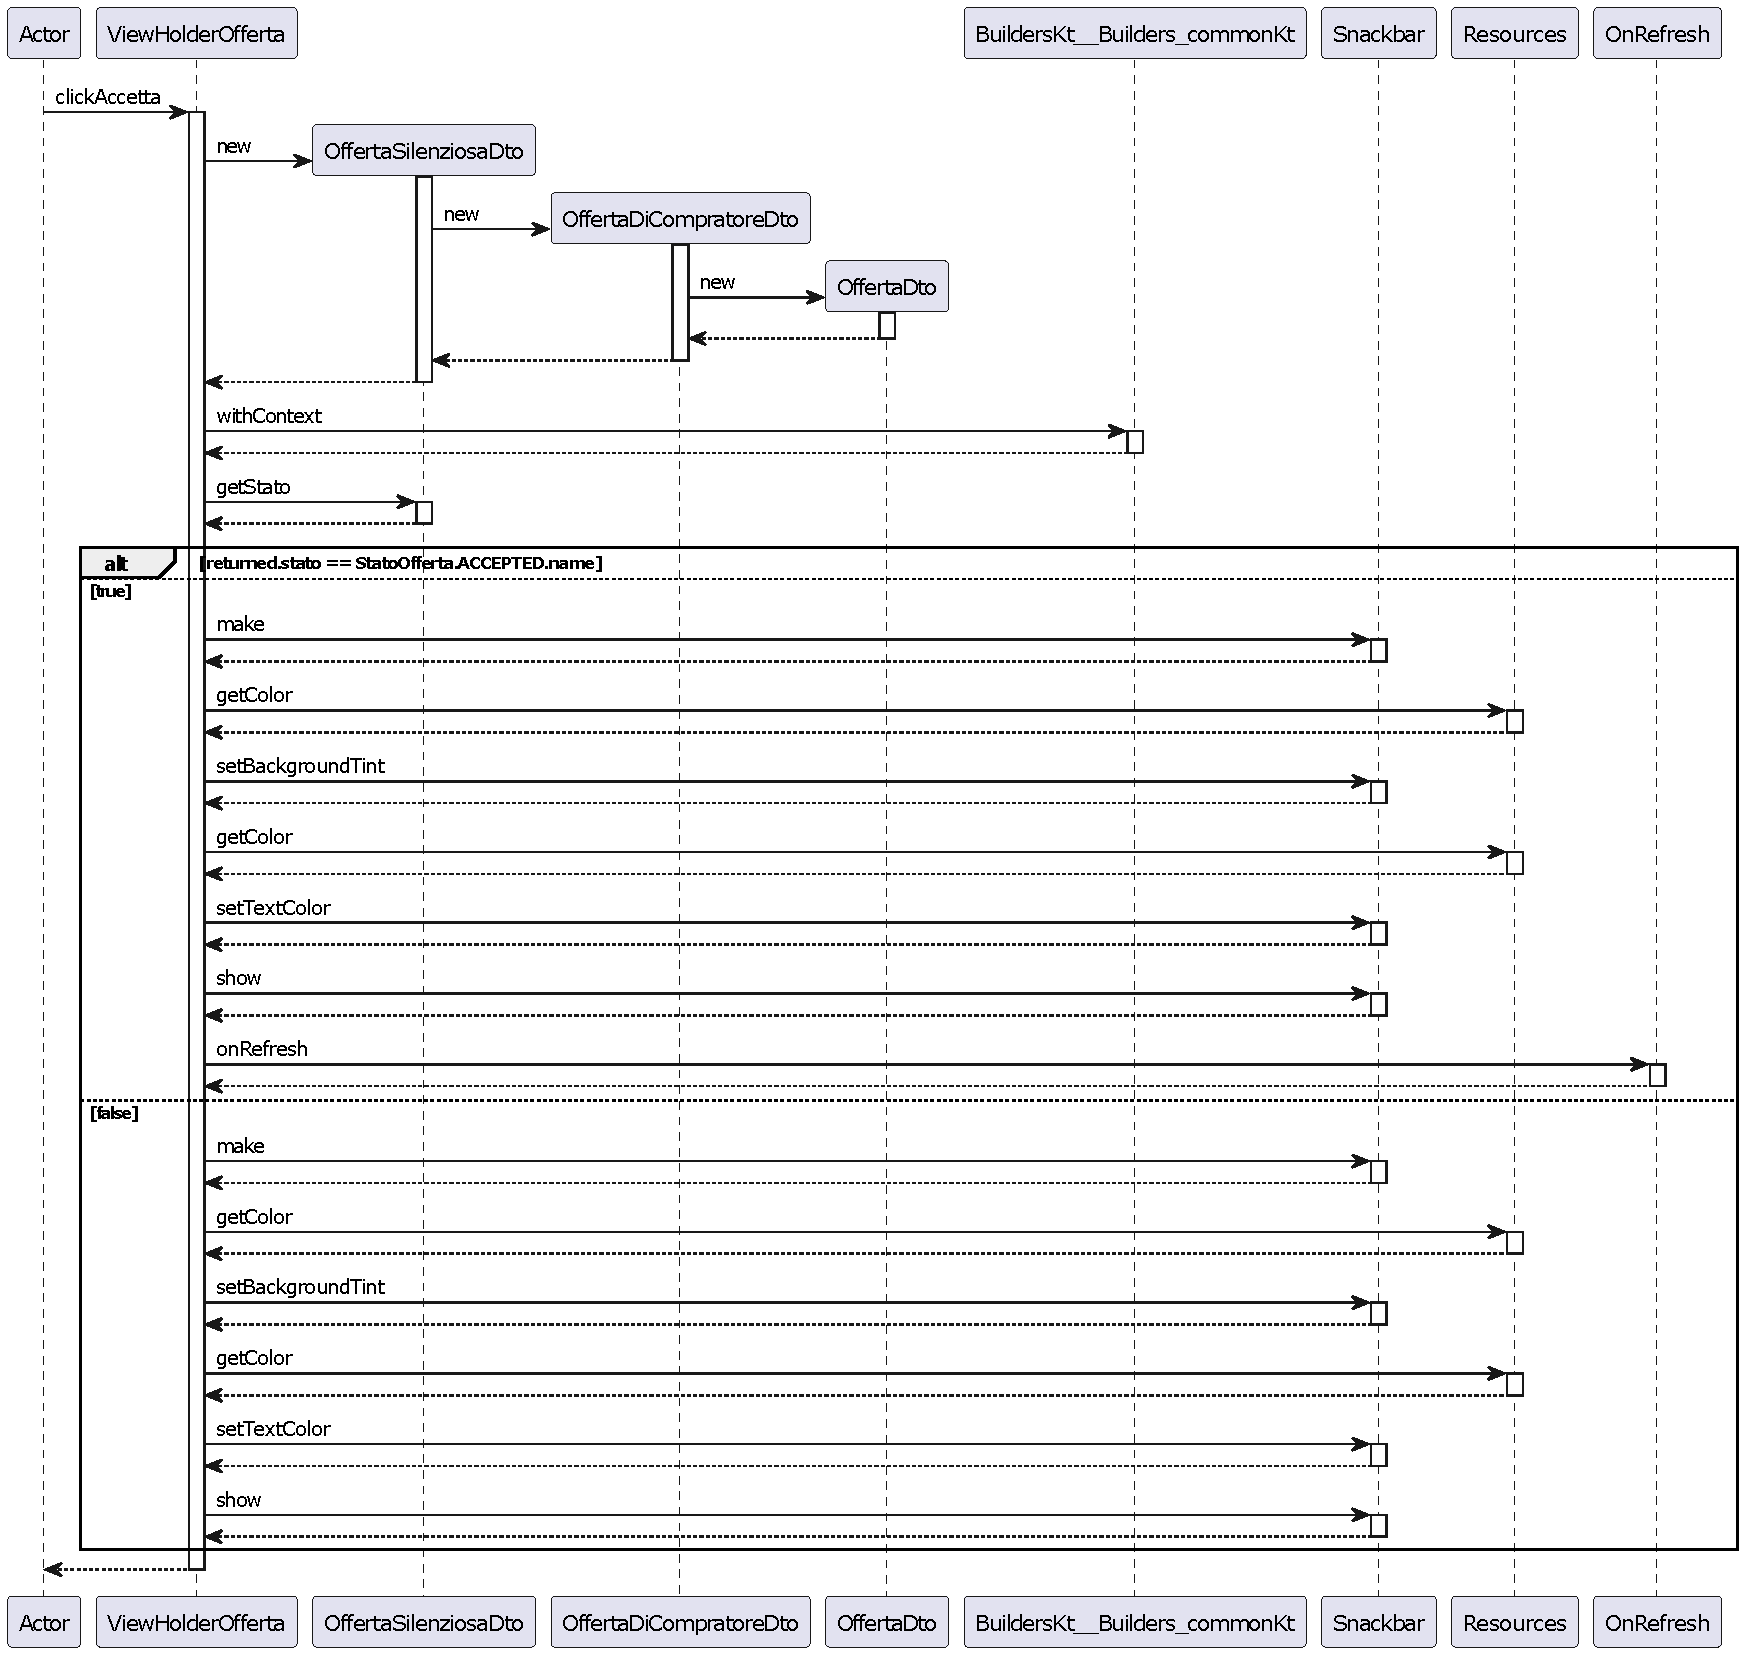
\includegraphics[width=1\linewidth]{Immagini/Diagrammi/Sequence Diagram/Design/Client Sequence Design/ClientSequenceAccettaOffertaDesign.pdf}
                \caption{Sequence Diagram di design accetta offerta per un'asta silenziosa (client)}
                \label{fig:Sequence Diagram di design accetta offerta per un'asta silenziosa (client)}
            \end{figure}

            \begin{figure}[htbp!]
                \centering
                    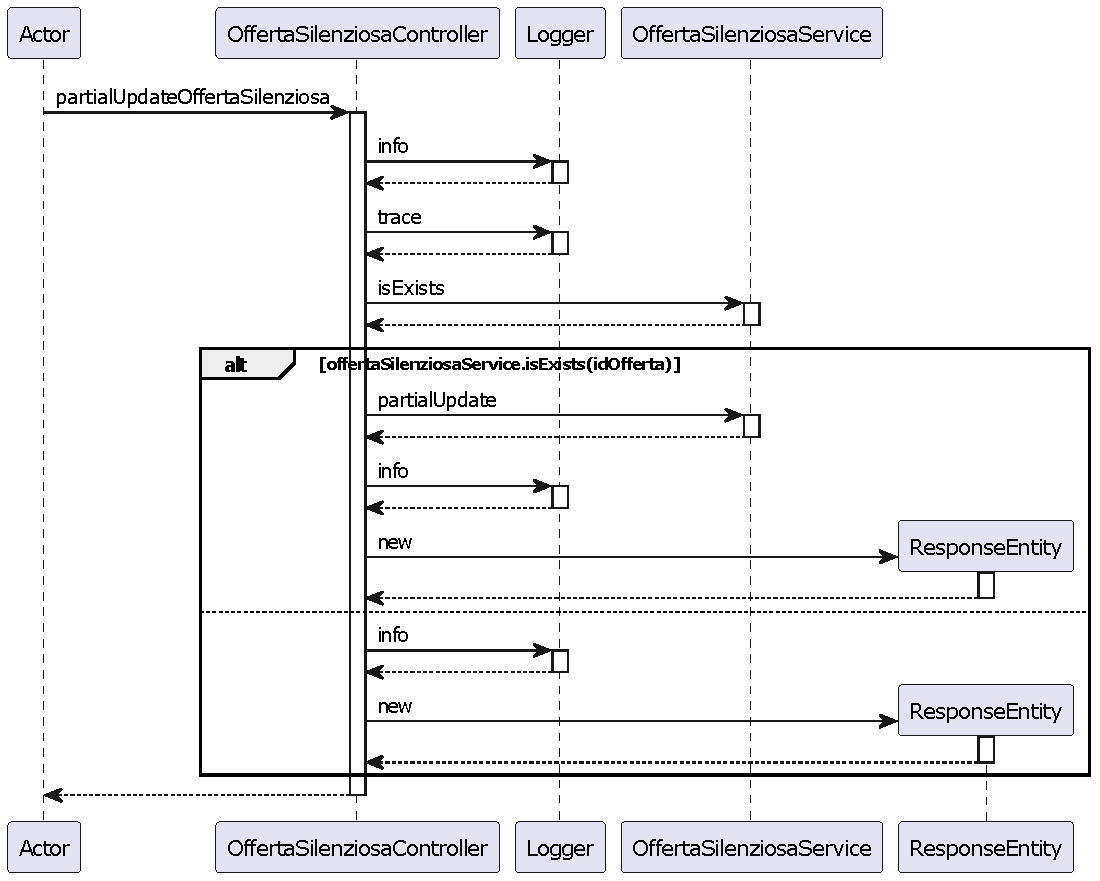
\includegraphics[width=1\linewidth]{Immagini/Diagrammi/Sequence Diagram/Design/Server Sequence Design/ServerSequenceAccettaOffertaDesign.pdf}
                \caption{Sequence Diagram di design accetta offerta per un'asta silenziosa (server)}
                \label{fig:Sequence Diagram di design accetta offerta per un'asta silenziosa (server)}
            \end{figure}

        \clearpage

        \subsection{III caso d'uso: Visualizza i dettagli di un'asta}
            \begin{figure}[htbp!]
                \centering
                    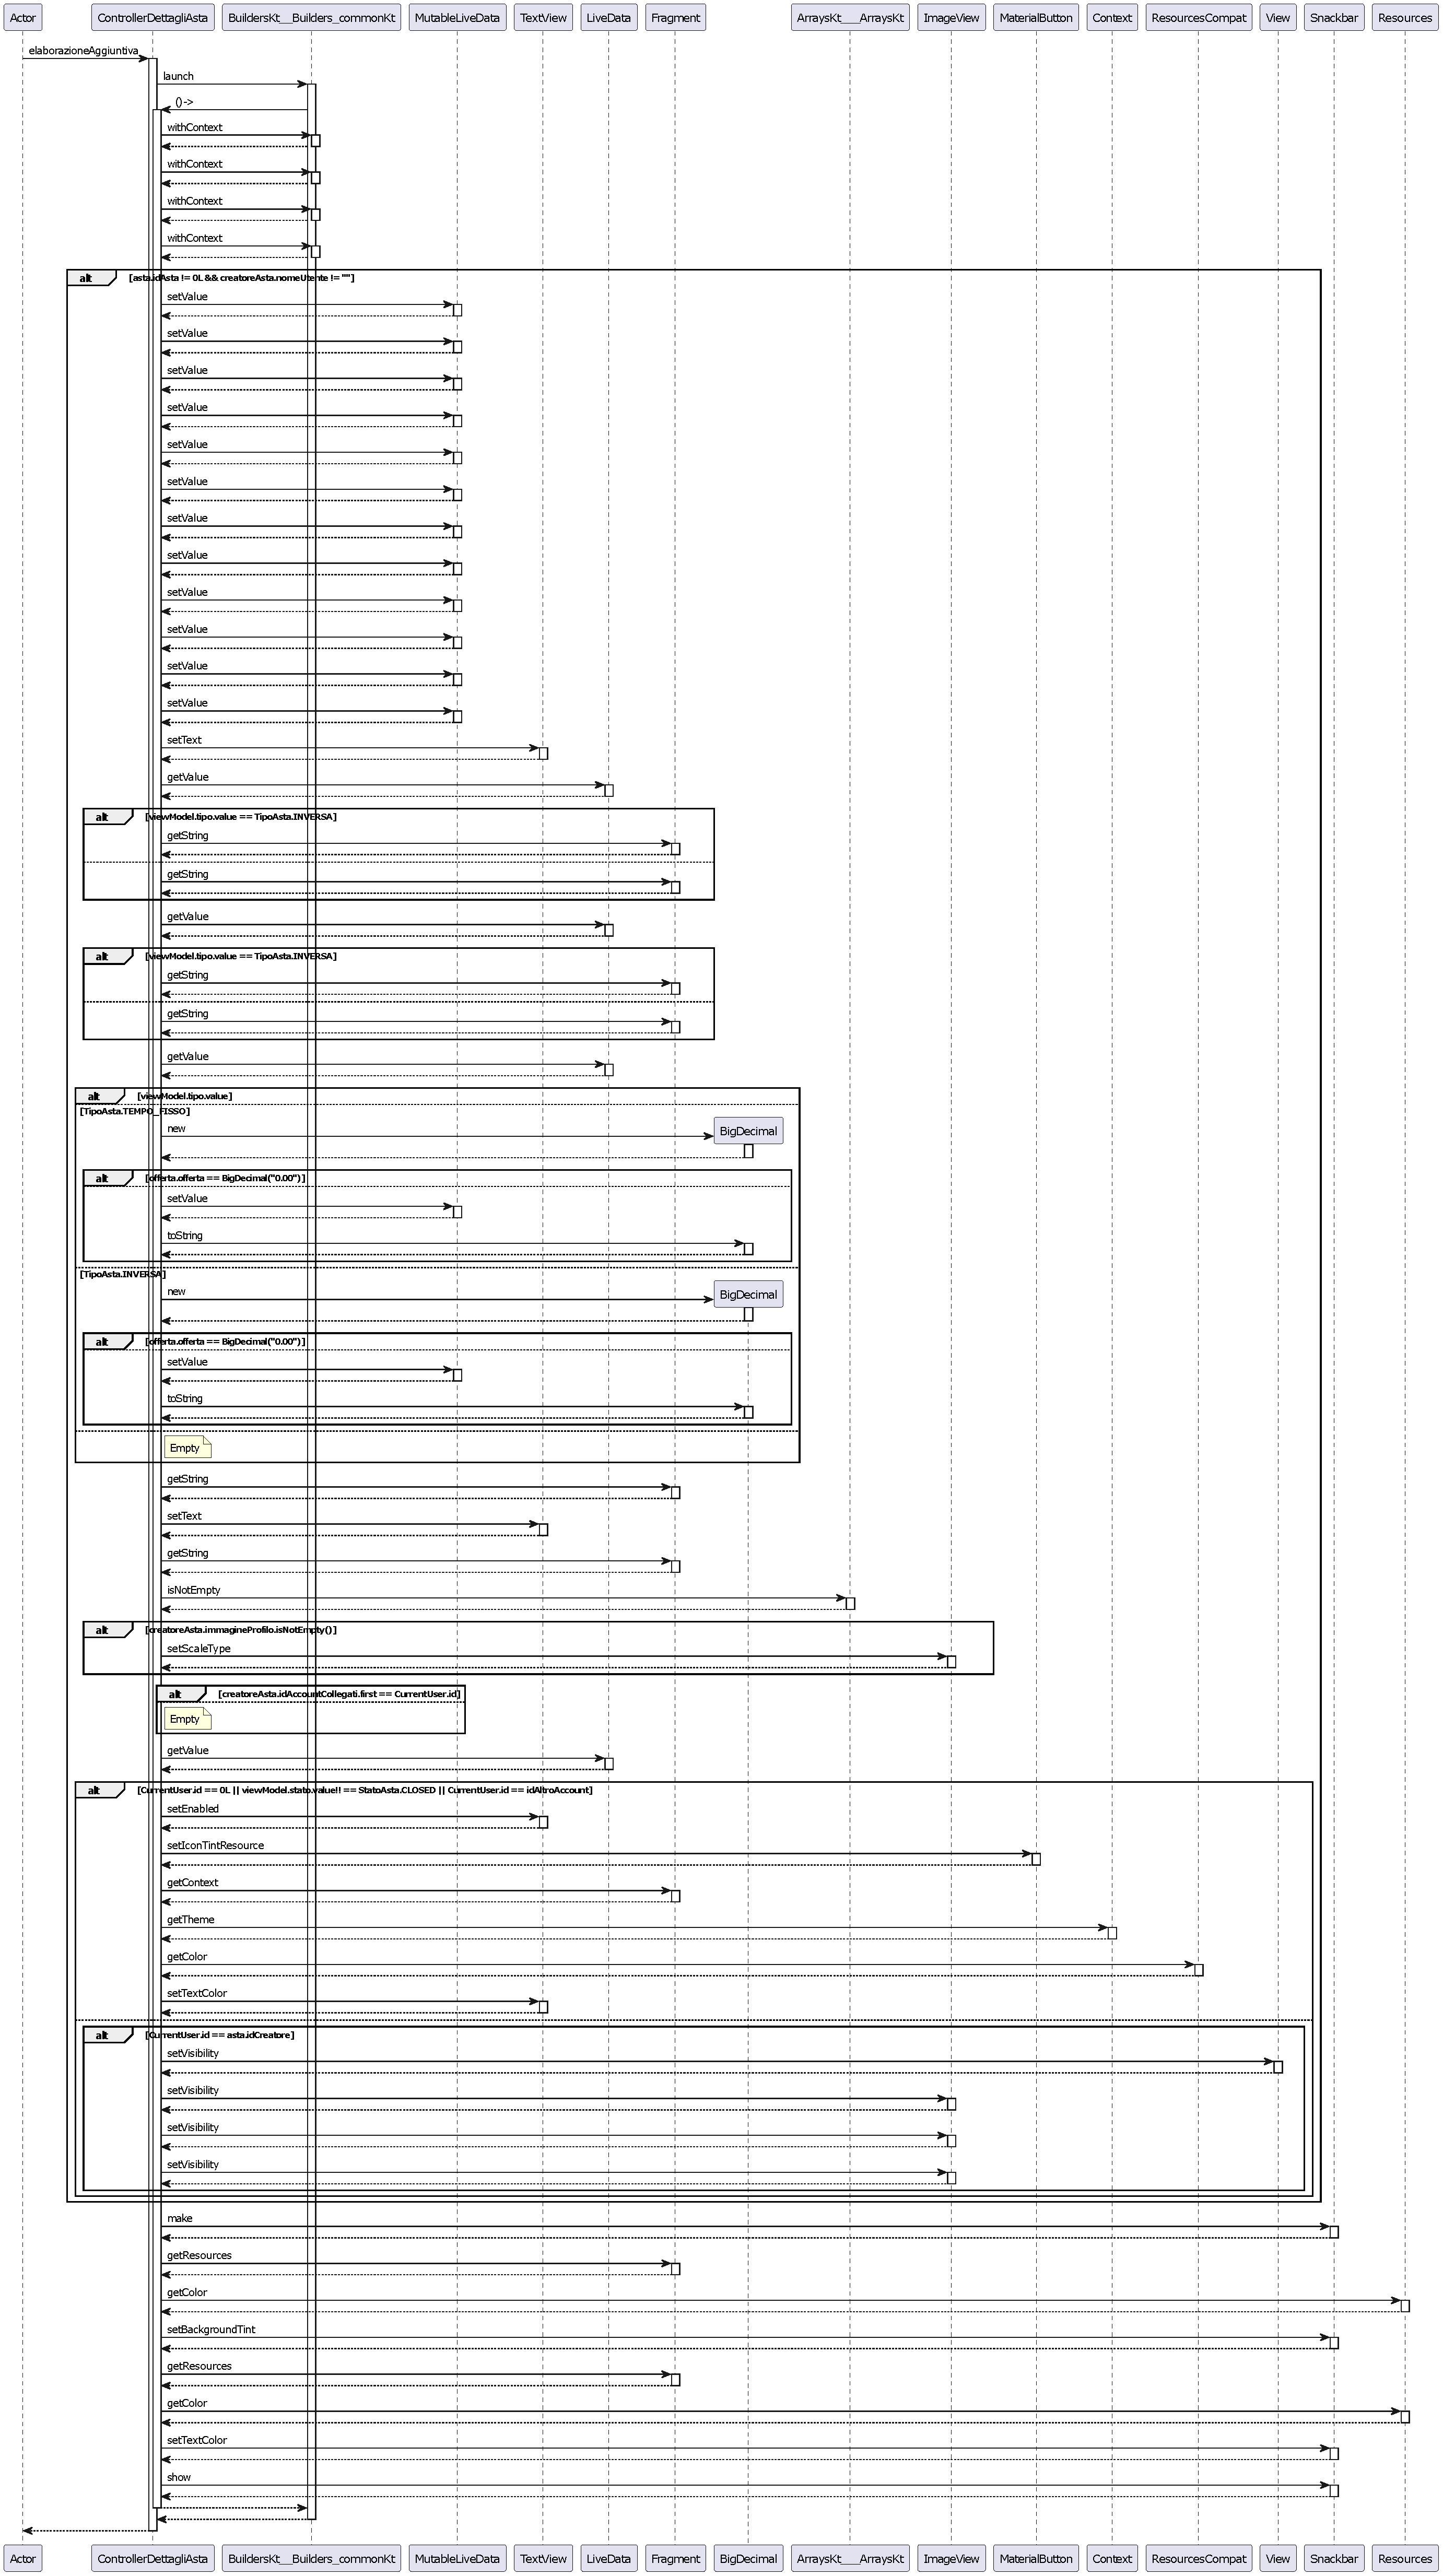
\includegraphics[width=0.71\linewidth]{Immagini/Diagrammi/Sequence Diagram/Design/Client Sequence Design/ClientSequenceDettagliAstaDesign.pdf}
                \caption{Sequence Diagram di design visualizza dettagli asta (client)}
                \label{fig:Sequence Diagram di design visualizza dettagli asta (client)}
            \end{figure}

            \begin{figure}[htbp!]
                \centering
                    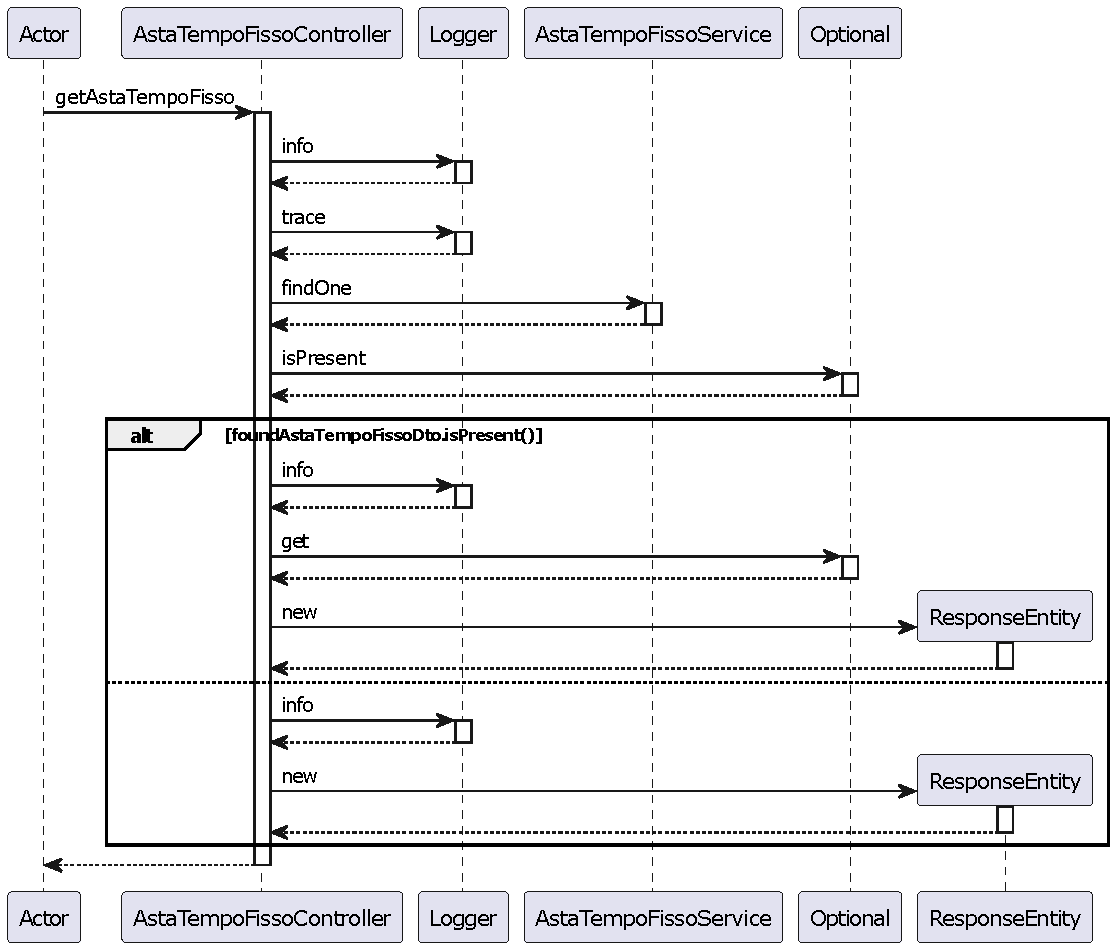
\includegraphics[width=1\linewidth]{Immagini/Diagrammi/Sequence Diagram/Design/Server Sequence Design/ServerSequenceDettagliAstaDesign.pdf}
                \caption{Sequence Diagram di design visualizza dettagli asta (server)}
                \label{fig:Sequence Diagram di design visualizza dettagli asta (server)}
            \end{figure}

        \clearpage

        \subsection{IV caso d'uso: Modificare il proprio profilo}
            \begin{figure}[htbp!]
                \centering
                    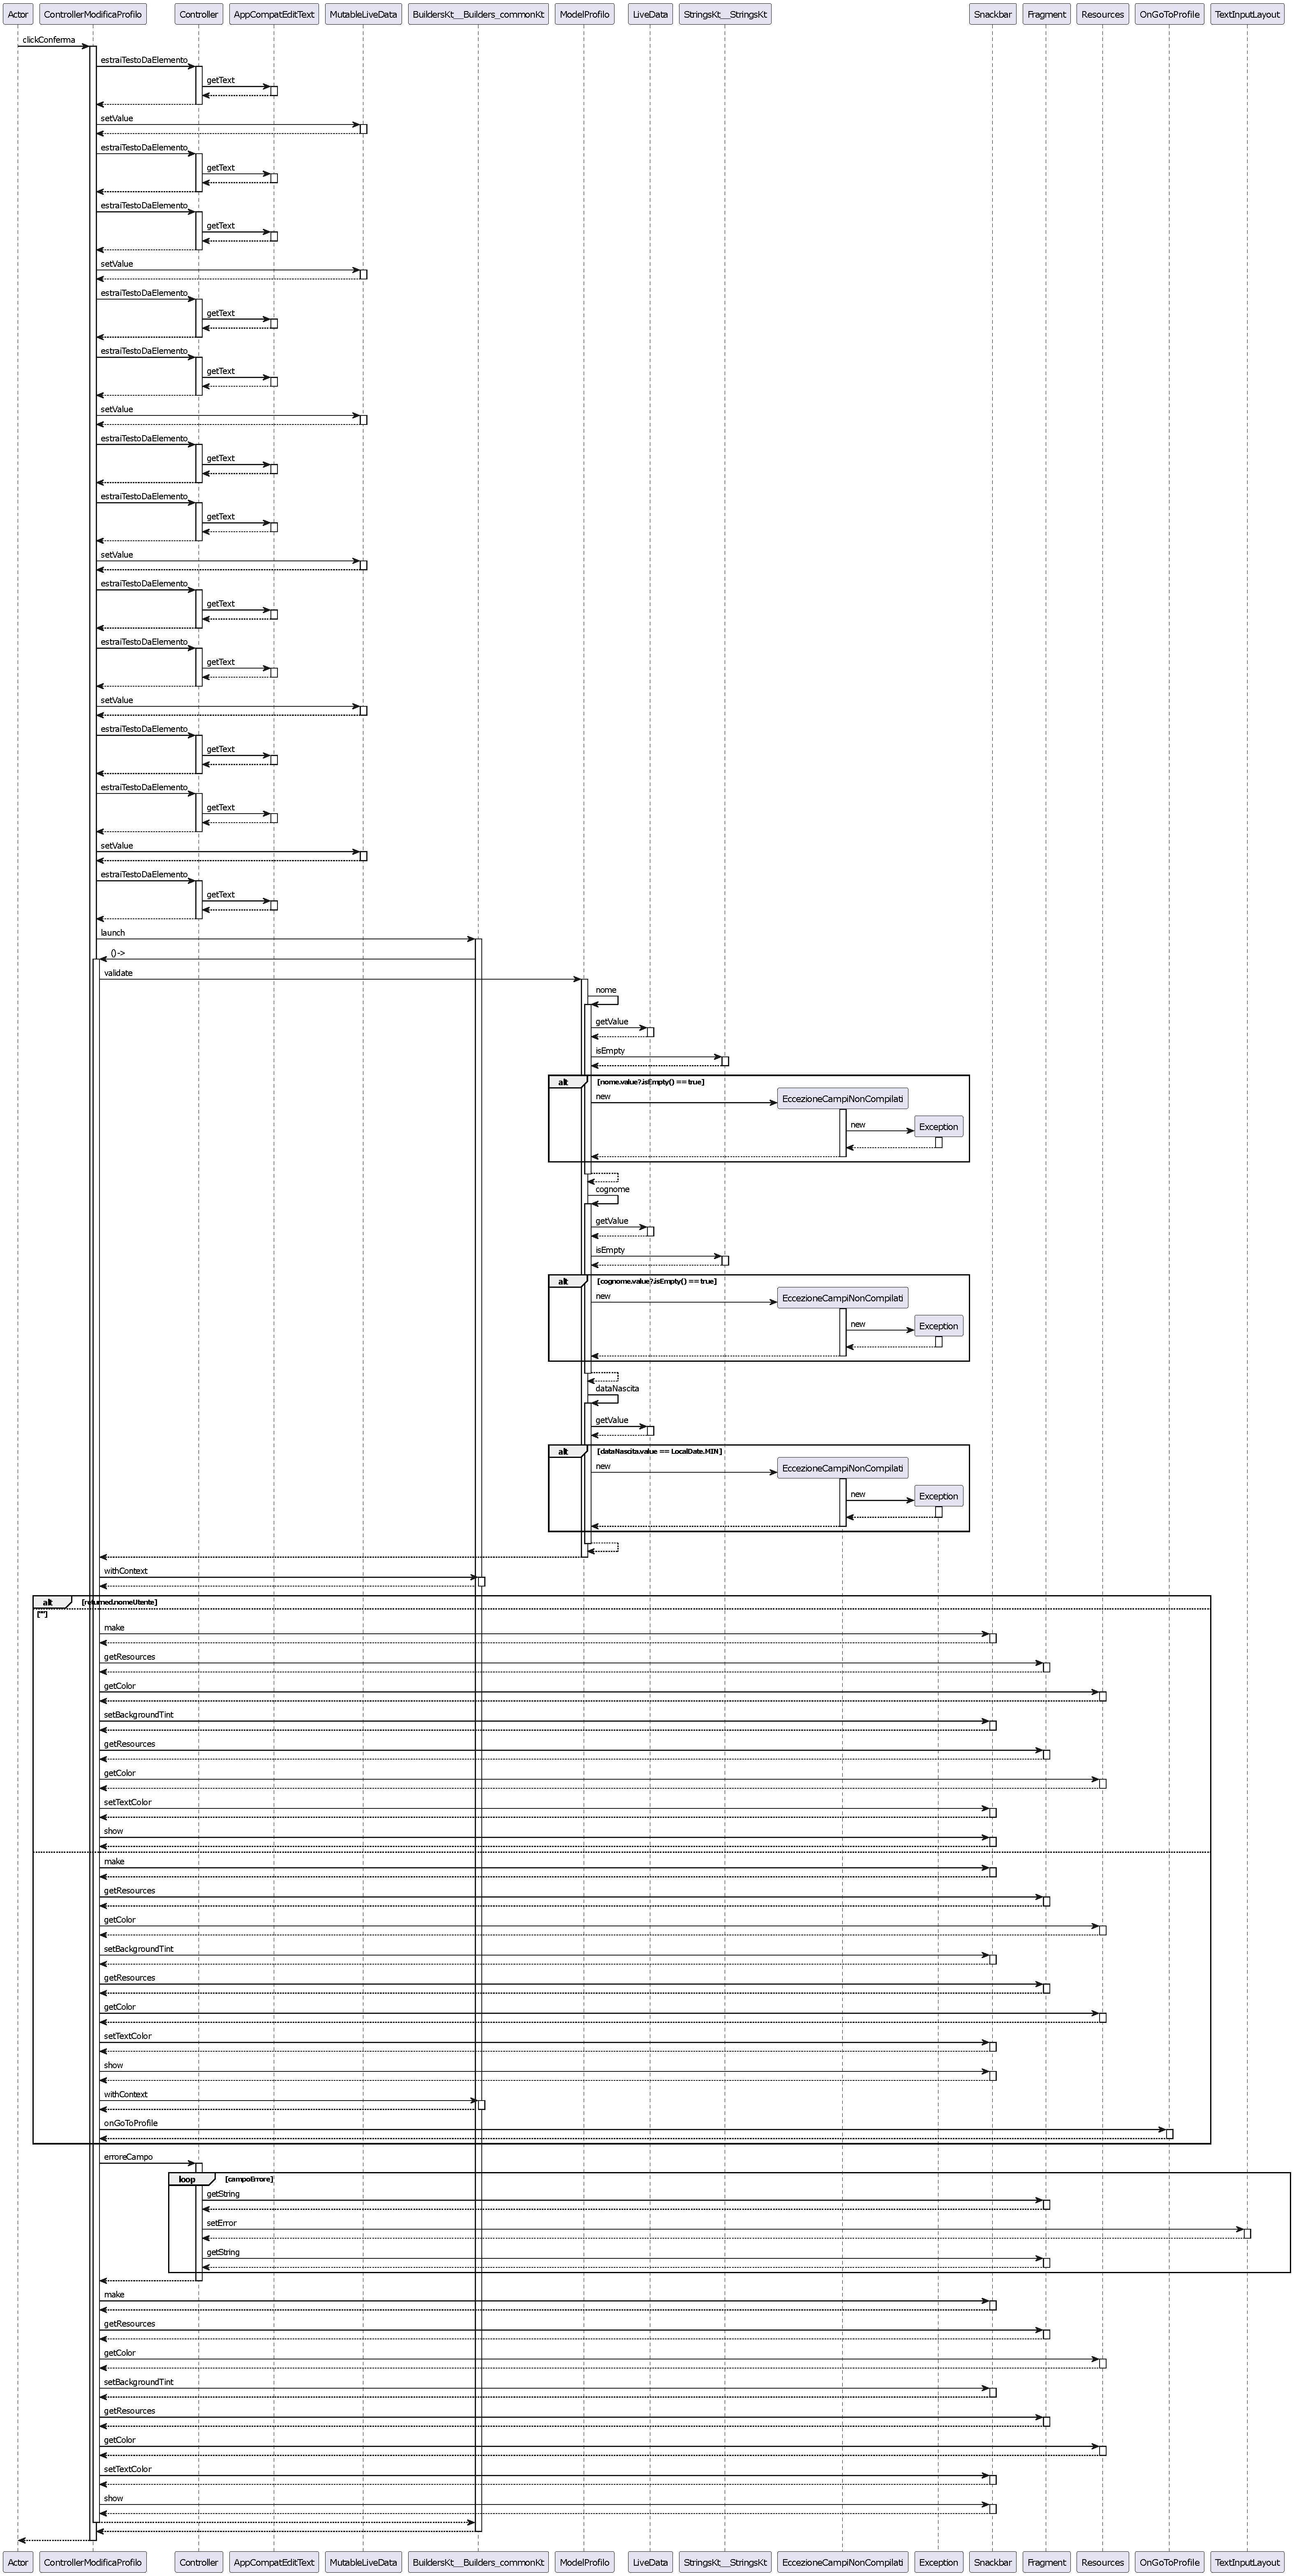
\includegraphics[width=0.64\linewidth]{Immagini/Diagrammi/Sequence Diagram/Design/Client Sequence Design/ClientSequenceModificaProfiloDesign.pdf}
                \caption{Sequence Diagram di design modifica dati profilo (client)}
                \label{fig:Sequence Diagram di design modifica dati profilo (client)}
            \end{figure}

            \begin{figure}[htbp!]
                \centering
                    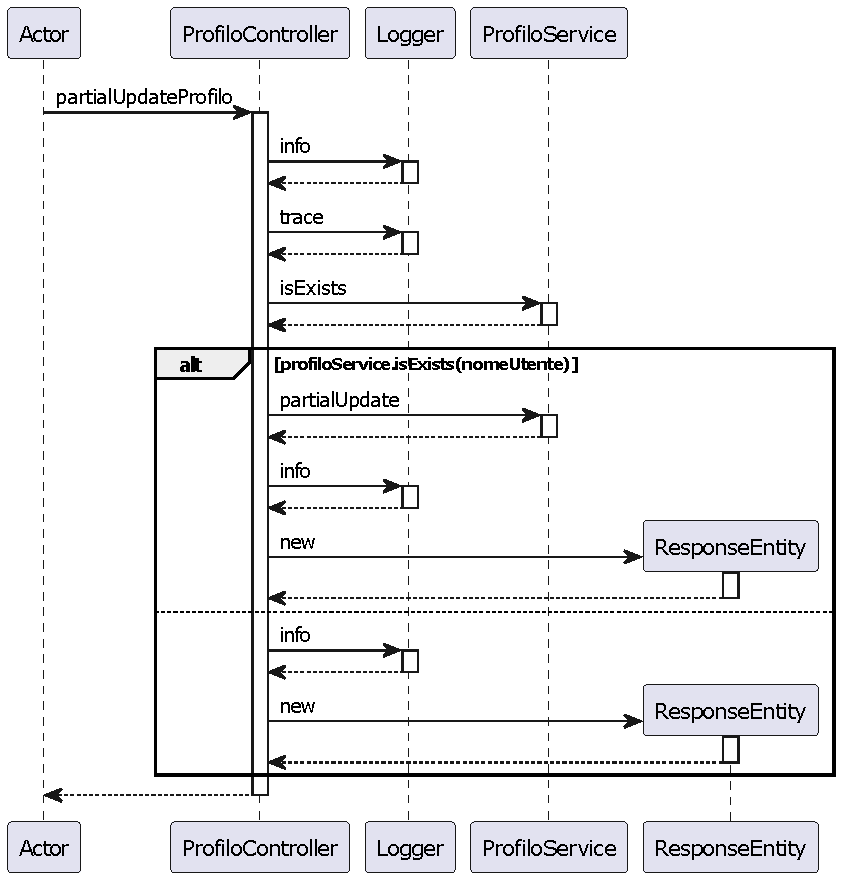
\includegraphics[width=1\linewidth]{Immagini/Diagrammi/Sequence Diagram/Design/Server Sequence Design/ServerSequenceModificaProfiloDesign.pdf}
                \caption{Sequence Diagram di design modifica dati profilo (server)}
                \label{fig:Sequence Diagram di design modifica dati profilo (server)}
            \end{figure}
    
    \clearpage

    \section{Endpoint}
        In questa sezione vengono descritti gli endpoints esposti dal backend. 
        
        NOTA: Gli endpoints che accettano query parameters, le ulteriori "modalità" sono separate da un ";".

        Per una descrizione dettagliata dei query parameters, esempi di richieste e di risposte per ciascun endpoint, riferirsi alla \href{https://documenter.getpostman.com/view/37147881/2sAYBd67Sj}{\underline{documentazione generata tramite Postman}}.
    
        \begin{longtable}{|C{4.2cm}|C{1.7cm}|L{6.2cm}|L{2.6cm}|}
                \hline
                    \cellcolor{head}\textbf{URI} &
                    \cellcolor{head}\textbf{METHOD} & \cellcolor{head}\textbf{DESCRIZIONE} &
                    \cellcolor{head}\textbf{AUTORIZZAZIONE MINIMA}\\
                \hline
                    \multirow[|c|]{5}{*}{/accounts/compratori}
                    & POST
                    & Permette di creare un account compratore
                    & USER \\
                \cline{2-4}
                    & GET
                    & Permette di recuperare tutti gli account compratori; filtrati per email; id
                    & ADMIN; USER; NO AUTH \\
                \cline{2-4}
                    & PUT
                    & Permette la sostituzione di un account compratore
                    & ADMIN \\
                \cline{2-4}
                    & PATCH
                    & Permette di modificare un campo "non associazione" di un account compratore
                    & ADMIN \\
                \cline{2-4}
                    & DELETE
                    & Permette di eliminare un account compratore
                    & ADMIN \\
                \hline
                    \multirow[|c|]{5}{*}{/accounts/venditori}
                    & POST
                    & Permette di creare un account venditore
                    & USER \\
                \cline{2-4}
                    & GET
                    & Permette di recuperare tutti gli account venditori; filtrati per email; id
                    & ADMIN; USER; NO AUTH \\
                \cline{2-4}
                    & PUT
                    & Permette la sostituzione di un account venditore
                    & ADMIN \\
                \cline{2-4}
                    & PATCH
                    & Permette di modificare un campo "non associazione" di un account venditore
                    & ADMIN \\
                \cline{2-4}
                    & DELETE
                    & Permette di eliminare un account venditore
                    & ADMIN \\
                \hline
                    \multirow[|c|]{5}{*}{/aste/di-compratori/inverse}
                    & POST
                    & Permette di creare un'asta inversa
                    & USER \\
                \cline{2-4}
                    & GET
                    & Permette di recuperare tutte le aste inverse; filtrate per nome e categoria; proprietario; offerente; id
                    & NO AUTH; NO AUTH; USER; USER; NO AUTH \\
                \cline{2-4}
                    & PUT
                    & Permette la sostituzione di un'asta inversa
                    & ADMIN \\
                \cline{2-4}
                    & PATCH
                    & Permette di modificare un campo "non associazione" di un'asta inversa
                    & USER \\
                \cline{2-4}
                    & DELETE
                    & Permette di eliminare un'asta inversa
                    & USER \\
                \hline
                    \multirow[|c|]{5}{*}{/aste/di-venditori/silenziose}
                    & POST
                    & Permette di creare un'asta silenziosa
                    & USER \\
                \cline{2-4}
                    & GET
                    & Permette di recuperare tutte le aste silenziose; filtrate per nome e categoria; proprietario; offerente; id
                    & NO AUTH; NO AUTH; USER; USER; NO AUTH \\
                \cline{2-4}
                    & PUT
                    & Permette la sostituzione di un'asta silenziosa
                    & ADMIN \\
                \cline{2-4}
                    & PATCH
                    & Permette di modificare un campo "non associazione" di un'asta silenziosa
                    & USER \\
                \cline{2-4}
                    & DELETE
                    & Permette di eliminare un'asta silenziosa
                    & USER \\
                \hline
                    \multirow[|c|]{5}{*}{/aste/di-venditori/tempo-fisso}
                    & POST
                    & Permette di creare un'asta a tempo fisso
                    & USER \\
                \cline{2-4}
                    & GET
                    & Permette di recuperare tutte le aste a tempo fisso; filtrate per nome e categoria; proprietario; offerente; id
                    & NO AUTH; NO AUTH; USER; USER; NO AUTH \\
                \cline{2-4}
                    & PUT
                    & Permette la sostituzione di un'asta a tempo fisso
                    & ADMIN \\
                \cline{2-4}
                    & PATCH
                    & Permette di modificare un campo "non associazione" di un'asta a tempo fisso
                    & USER \\
                \cline{2-4}
                    & DELETE
                    & Permette di eliminare un'asta a tempo fisso
                    & USER \\
                \hline
                    \multirow[|c|]{5}{*}{/offerte/di-compratori/tempo-fisso}
                    & POST
                    & Permette di creare un'offerta a tempo fisso
                    & USER \\
                \cline{2-4}
                    & GET
                    & Permette di recuperare tutte le offerte a tempo fisso; filtrate per asta di riferimento; maggior valore e asta riferimento; maggior valore, asta riferimento e venditore; id
                    & ADMIN; USER; NO AUTH; USER; ADMIN \\
                \cline{2-4}
                    & PUT
                    & Permette la sostituzione di un'offerta a tempo fisso
                    & ADMIN \\
                \cline{2-4}
                    & PATCH
                    & Permette di modificare un campo "non associazione" di un'offerta a tempo fisso
                    & ADMIN \\
                \cline{2-4}
                    & DELETE
                    & Permette di eliminare un'offerta a tempo fisso
                    & ADMIN \\
                \hline
                    \multirow[|c|]{5}{*}{/offerte/di-compratori/silenziose}
                    & POST
                    & Permette di creare un'offerta silenziosa
                    & USER \\
                \cline{2-4}
                    & GET
                    & Permette di recuperare tutte le offerte silenziose; filtrate per asta di riferimento; maggior valore e asta riferimento; maggior valore, asta riferimento e venditore; id
                    & ADMIN; USER; NO AUTH; USER; ADMIN \\
                \cline{2-4}
                    & PUT
                    & Permette la sostituzione di un'offerta silenziosa
                    & ADMIN \\
                \cline{2-4}
                    & PATCH
                    & Permette di modificare un campo "non associazione" di un'offerta silenziosa
                    & USER \\
                \cline{2-4}
                    & DELETE
                    & Permette di eliminare un'offerta silenziosa
                    & ADMIN \\
                \hline
                    \multirow[|c|]{5}{*}{/offerte/di-venditori/inverse}
                    & POST
                    & Permette di creare un'offerta inversa
                    & USER \\
                \cline{2-4}
                    & GET
                    & Permette di recuperare tutte le offerte inverse; filtrate per asta di riferimento; maggior valore e asta riferimento; maggior valore, asta riferimento e venditore; id
                    & ADMIN; USER; NO AUTH; USER; ADMIN \\
                \cline{2-4}
                    & PUT
                    & Permette la sostituzione di un'offerta inversa
                    & ADMIN \\
                \cline{2-4}
                    & PATCH
                    & Permette di modificare un campo "non associazione" di un'offerta inversa
                    & ADMIN \\
                \cline{2-4}
                    & DELETE
                    & Permette di eliminare un'offerta inversa
                    & ADMIN \\
                \hline
                    \multirow[|c|]{4}{*}{/categorie-asta}
                    & PUT
                    & Permette di creare (o sostituire, se già esistente) una categoria asta
                    & ADMIN \\
                \cline{2-4}
                    & GET
                    & Permette di recuperare tutte le categorie asta; filtrate per id
                    & NO AUTH; NO AUTH \\
                \cline{2-4}
                    & PATCH
                    & Permette di modificare un campo "non associazione" di una categoria asta
                    & ADMIN \\
                \cline{2-4}
                    & DELETE
                    & Permette di eliminare una categoria asta
                    & ADMIN \\
                \hline
                    \multirow[|c|]{5}{*}{/notifiche}
                    & POST
                    & Permette di creare una notifica
                    & ADMIN \\
                \cline{2-4}
                    & GET
                    & Permette di recuperare tutte le notifiche; filtrate per destinatario; id
                    & ADMIN; USER; ADMIN \\
                \cline{2-4}
                    & PUT
                    & Permette la sostituzione di una notifica
                    & ADMIN \\
                \cline{2-4}
                    & PATCH
                    & Permette di modificare un campo "non associazione" di una notifica
                    & ADMIN \\
                \cline{2-4}
                    & DELETE
                    & Permette di eliminare una notifica
                    & ADMIN \\
                \hline
                    \multirow[|c|]{4}{*}{/profili}
                    & PUT
                    & Permette di creare (o sostituire, se già esistente) un profilo. Viene automaticamente creato un account associato
                    & USER \\
                \cline{2-4}
                    & GET
                    & Permette di recuperare tutti i profili; filtrati per id
                    & ADMIN; NO AUTH \\
                \cline{2-4}
                    & PATCH
                    & Permette di modificare un campo "non associazione" di un profilo
                    & USER \\
                \cline{2-4}
                    & DELETE
                    & Permette di eliminare un profilo
                    & ADMIN \\
                \hline
                    /auth/url
                    & GET
                    & Permette di recuperare l'URL a cui collegarsi per fare l'autenticazione
                    & NO AUTH \\
                \hline
                    /auth/callback
                    & GET
                    & Permette di autenticare un account in base al codice restituito dal provider di autenticazione
                    & NO AUTH \\
                \hline
                    /auth/refresh
                    & GET
                    & Permette di aggiornare la sessione di autenticazione tramite il refresh\_token restituito da auth/callback
                    & NO AUTH \\
                \hline
                    /auth/logout
                    & GET
                    & Permette di eliminare la sessione di autenticazione tramite il refresh\_token restituito da auth/callback e restituisce l'URL a cui accedere per dimenticare le credenziali di login
                    & USER \\
                \hline
            \end{longtable}

    \clearpage
    
    \section{Database}
        L'analisi dei requisiti permette di individuare le entità, relazioni ed attributi che caratterizzano il dominio del problema. Tuttavia, per immagazzinare questi dati in una base di dati relazionale in modo efficace è necessario fare uno studio adeguato al fine di arrivare a uno schema di base di dati che permetta di rispettare i requisiti non funzionali di velocità ed efficienza.
    
        \subsection{Ristrutturazione della progettazione concettuale}
            \begin{figure}[htbp!]
                \centering
                    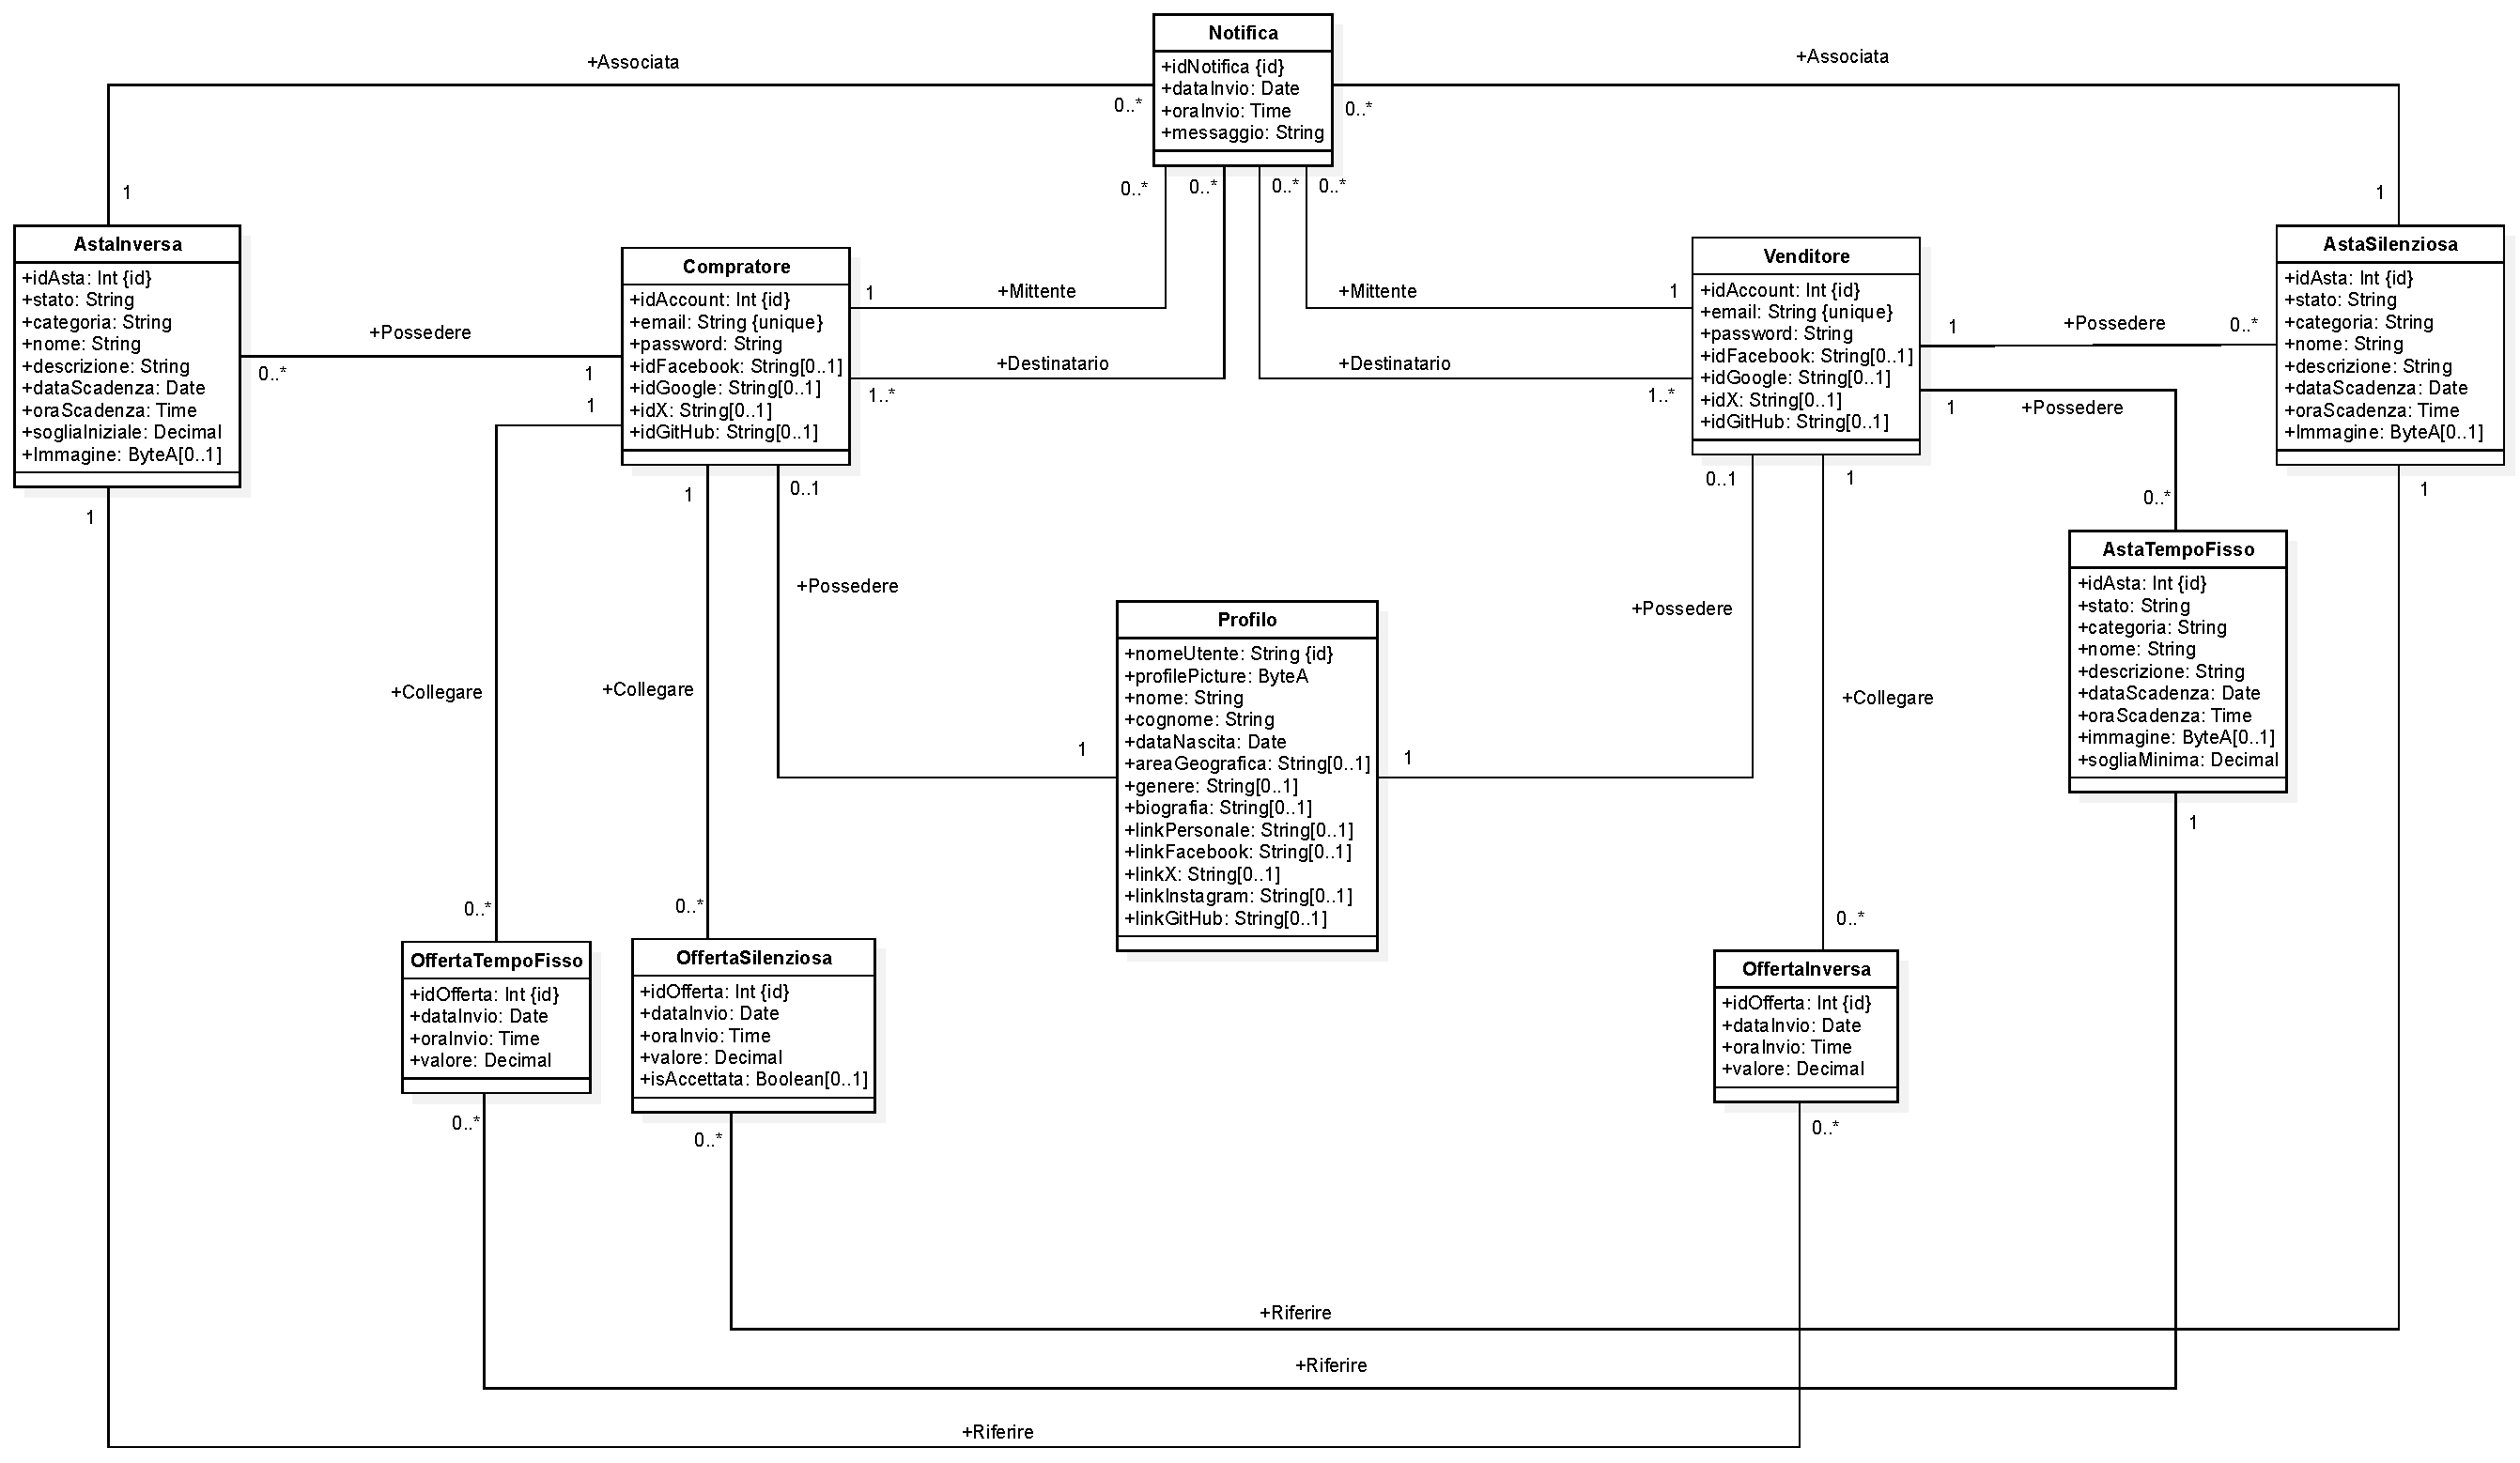
\includegraphics[width=0.73\linewidth]{Immagini/Diagrammi/Class Diagram/Design/ClassDiagramDatabaseRistrutturato.pdf}
                \caption{Schema concettuale ristrutturato del database}
                \label{fig:Schema concettuale ristrutturato del database}
            \end{figure}
            
        \subsection{Schema logico}
            \begin{figure}[htbp!]
                \centering
                    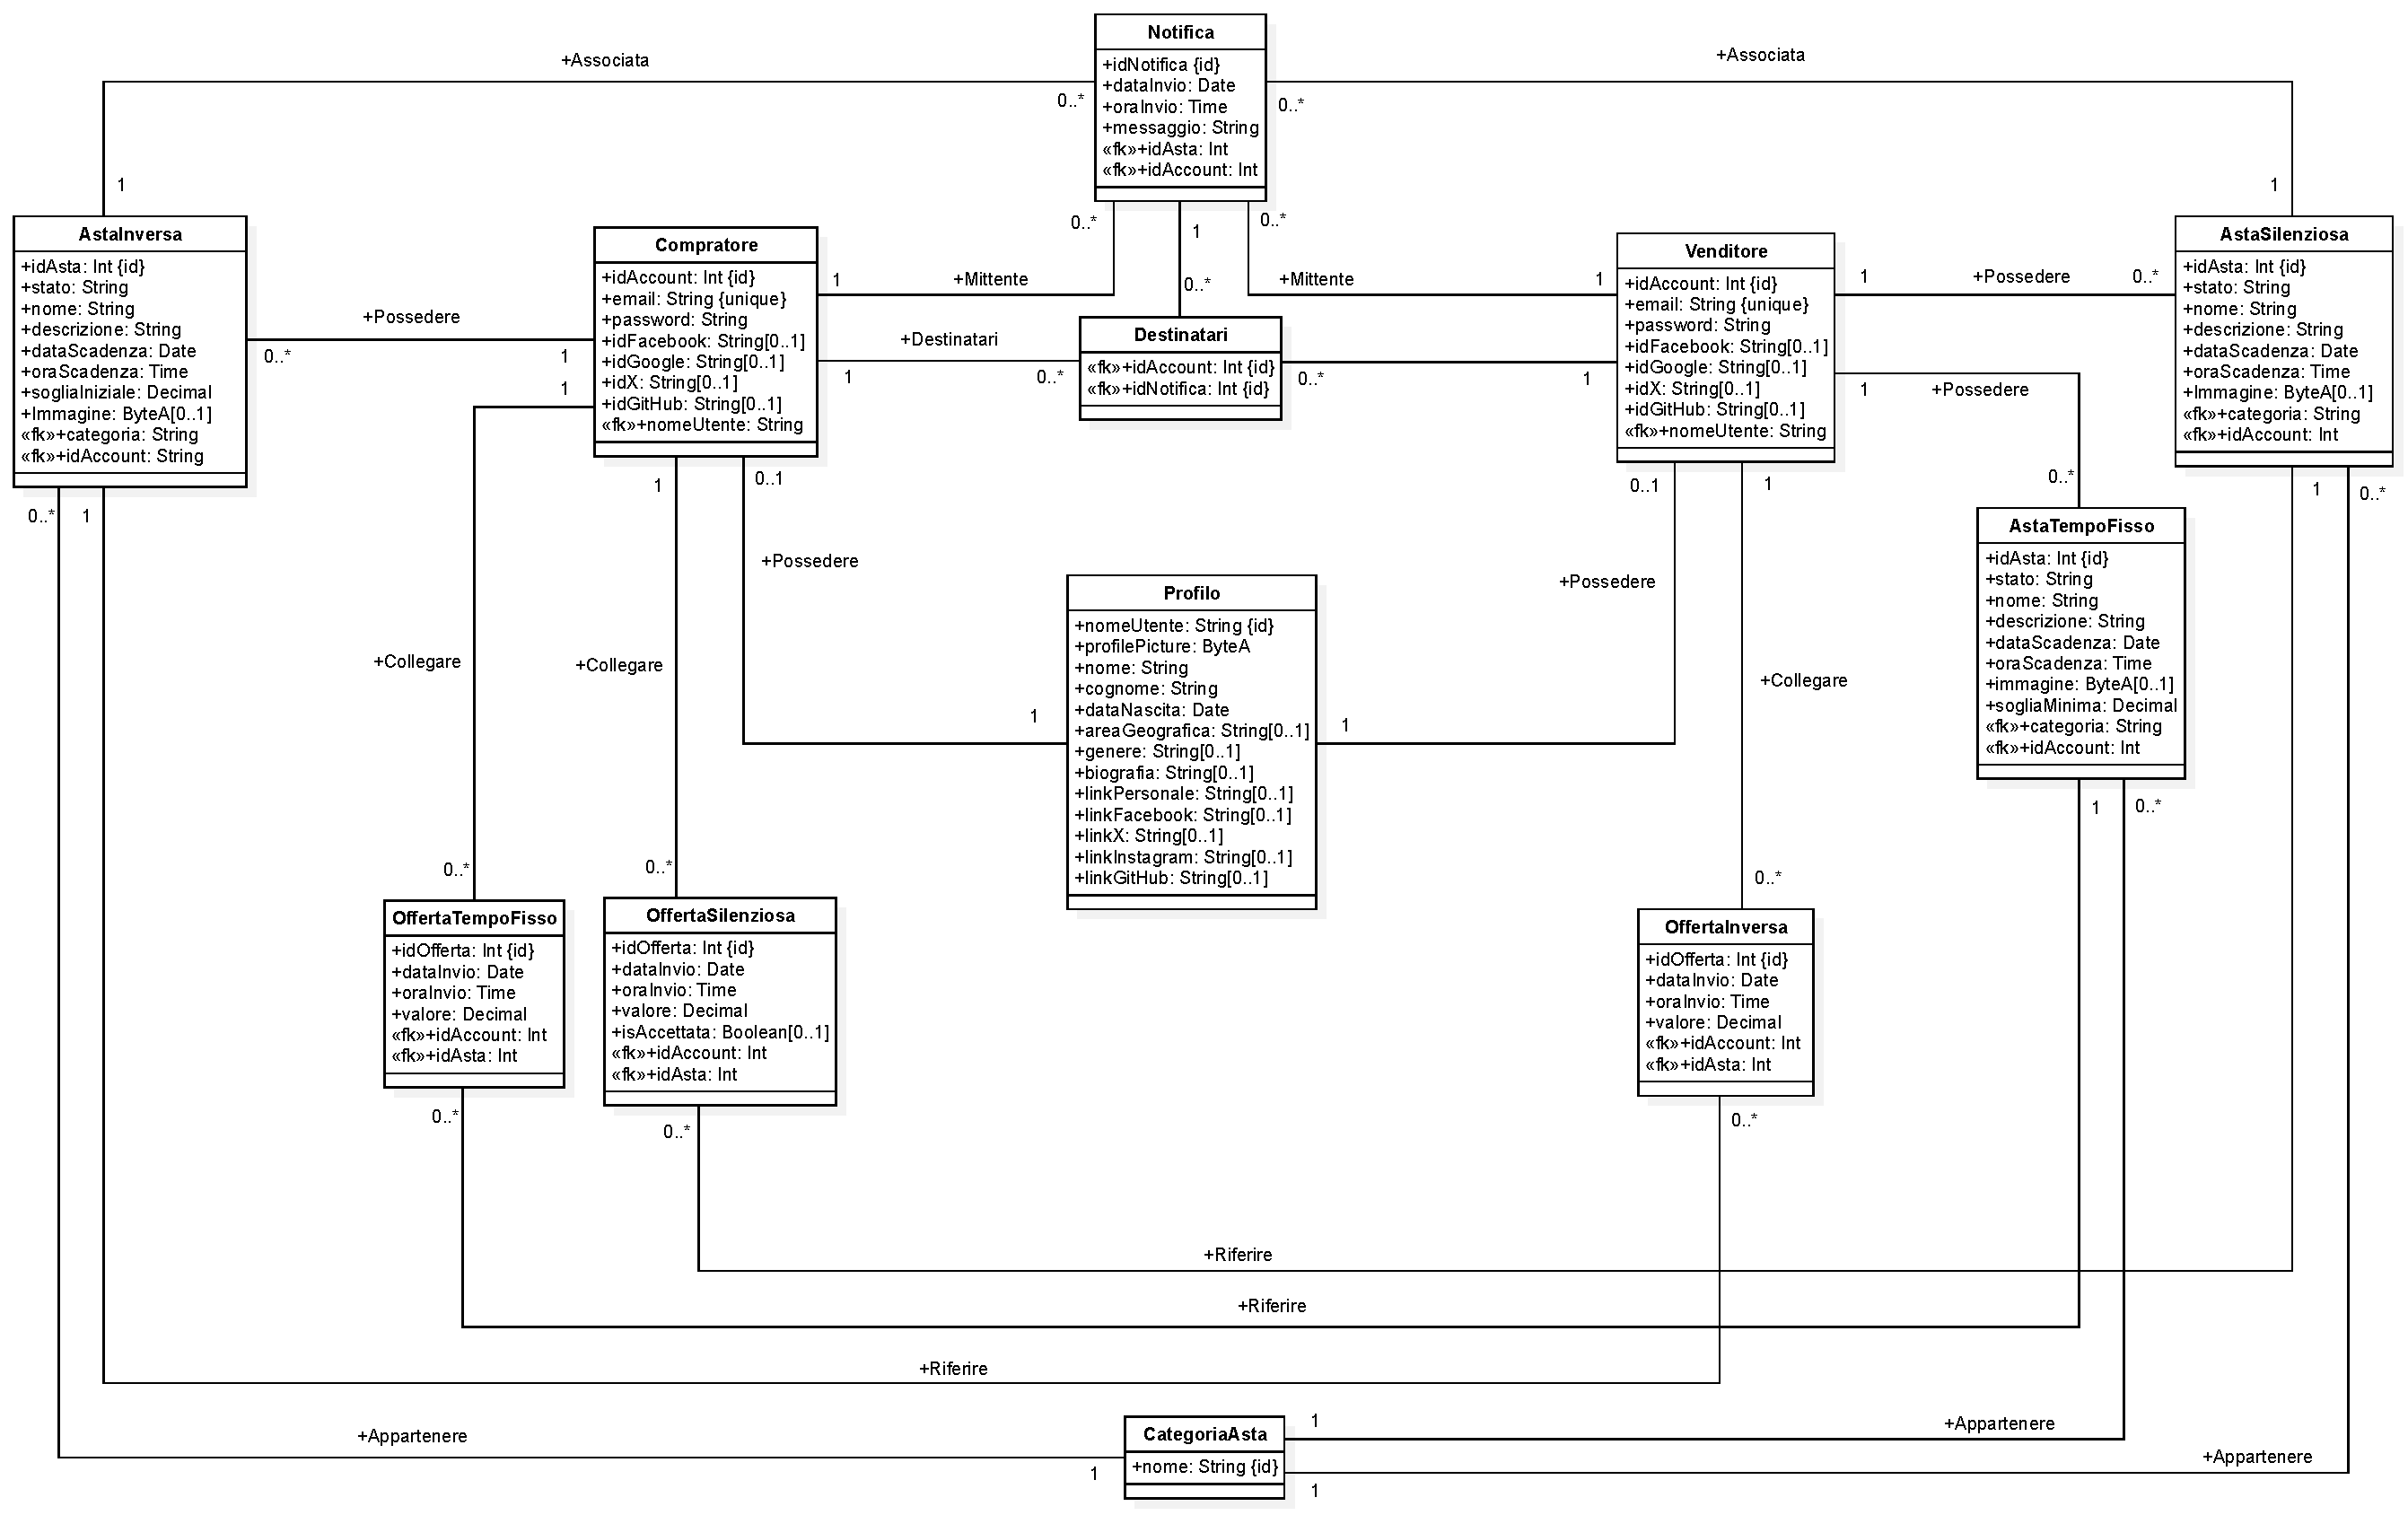
\includegraphics[width=0.73\linewidth]{Immagini/Diagrammi/Class Diagram/Design/ClassDiagramDatabaseLogico.pdf}
                \caption{Schema logico del database}
                \label{fig:Schema logico del database}
            \end{figure}

        \clearpage
        
        \subsection{Schema fisico}
            \begin{lstlisting}[language=SQL, caption=Preparazione ambiente]
                DROP SCHEMA IF EXISTS dd24 CASCADE;
                CREATE SCHEMA dd24;
                SET search_path TO dd24;
            \end{lstlisting}
                        
            \begin{lstlisting}[language=SQL, caption=Relazione categoria asta]
                CREATE TABLE categoria_asta
                (
                    nome TEXT NOT NULL,
                    CONSTRAINT pk_categoria_asta PRIMARY KEY (nome)
                );
            \end{lstlisting}
            
            \begin{lstlisting}[language=SQL, caption=Relazione profilo]
                CREATE TABLE profilo
                (
                    nome_utente     TEXT NOT NULL,
                    CONSTRAINT pk_profilo PRIMARY KEY (nome_utente),
                    area_geografica TEXT,
                    biografia       TEXT,
                    cognome         TEXT NOT NULL,
                    data_nascita    DATE NOT NULL,
                    CONSTRAINT chk_data_nascita CHECK (data_nascita <= NOW()),
                    genere          TEXT NOT NULL,
                    nome            TEXT NOT NULL,
                    link_personale  TEXT,
                    link_facebook   TEXT,
                    link_x          TEXT,
                    link_instagram  TEXT,
                    link_git_hub    TEXT,
                    profile_picture BYTEA
                );
            \end{lstlisting}
            
            \begin{lstlisting}[language=SQL, caption=Relazione compratore]
                CREATE TABLE compratore
                (
                    id_account          BIGSERIAL NOT NULL,
                    CONSTRAINT pk_compratore PRIMARY KEY (id_account),
                    email               TEXT      NOT NULL,
                    CONSTRAINT uk_compratore_email UNIQUE (email),
                    password            TEXT      NOT NULL,
                    id_facebook         TEXT,
                    id_git_hub          TEXT,
                    id_google           TEXT,
                    id_x                TEXT,
                    profilo_nome_utente TEXT      NOT NULL,
                    CONSTRAINT fk_profilo_nome_utente FOREIGN KEY (profilo_nome_utente) REFERENCES profilo (nome_utente) ON UPDATE CASCADE ON DELETE CASCADE
                );
                
                CREATE FUNCTION cleanup_compratore()
                    RETURNS TRIGGER AS
                $$
                BEGIN
                    DELETE
                    FROM offerta_silenziosa
                    WHERE compratore_id_account = OLD.id_account;
                    DELETE
                    FROM offerta_tempo_fisso
                    WHERE compratore_id_account = OLD.id_account;
                    DELETE
                    FROM asta_inversa
                    WHERE compratore_id_account = OLD.id_account;
                    DELETE
                    FROM destinatari
                    WHERE account_id_account = OLD.id_account;
                    DELETE
                    FROM notifica
                    WHERE account_id_account = OLD.id_account;
                END
                $$
                    LANGUAGE PLPGSQL;
                
                CREATE TRIGGER trg_compratore
                    BEFORE DELETE
                    ON compratore
                    FOR EACH ROW
                EXECUTE FUNCTION cleanup_compratore();
            \end{lstlisting}
            
            \begin{lstlisting}[language=SQL, caption=Relazione venditore]
                CREATE TABLE venditore
                (
                    id_account          BIGSERIAL NOT NULL,
                    CONSTRAINT pk_venditore PRIMARY KEY (id_account),
                    email               TEXT      NOT NULL,
                    CONSTRAINT uk_venditore_email UNIQUE (email),
                    password            TEXT      NOT NULL,
                    id_facebook         TEXT,
                    id_git_hub          TEXT,
                    id_google           TEXT,
                    id_x                TEXT,
                    profilo_nome_utente TEXT      NOT NULL,
                    CONSTRAINT fk_profilo_nome_utente FOREIGN KEY (profilo_nome_utente) REFERENCES profilo (nome_utente) ON UPDATE CASCADE ON DELETE CASCADE
                );
                
                CREATE FUNCTION cleanup_venditore()
                    RETURNS TRIGGER AS
                $$
                BEGIN
                    DELETE
                    FROM offerta_inversa
                    WHERE venditore_id_account = OLD.id_account;
                    DELETE
                    FROM asta_tempo_fisso
                    WHERE venditore_id_account = OLD.id_account;
                    DELETE
                    FROM asta_silenziosa
                    WHERE venditore_id_account = OLD.id_account;
                    DELETE
                    FROM destinatari
                    WHERE account_id_account = OLD.id_account;
                    DELETE
                    FROM notifica
                    WHERE account_id_account = OLD.id_account;
                END
                $$
                    LANGUAGE PLPGSQL;
                
                CREATE TRIGGER trg_venditore
                    BEFORE DELETE
                    ON venditore
                    FOR EACH ROW
                EXECUTE FUNCTION cleanup_venditore();
            \end{lstlisting}
            
            \begin{lstlisting}[language=SQL, caption=Relazione asta inversa]
                CREATE TABLE asta_inversa
                (
                    id_asta               BIGSERIAL      NOT NULL,
                    CONSTRAINT pk_asta_inversa PRIMARY KEY (id_asta),
                    data_scadenza         DATE           NOT NULL,
                    CONSTRAINT chk_data_scadenza CHECK (data_scadenza > NOW()),
                    descrizione           TEXT           NOT NULL,
                    immagine              BYTEA,
                    nome                  TEXT           NOT NULL,
                    ora_scadenza          TIME           NOT NULL,
                    categoria_asta_nome   TEXT           NOT NULL,
                    CONSTRAINT fk_categoria_asta_nome FOREIGN KEY (categoria_asta_nome) REFERENCES categoria_asta (nome) ON UPDATE CASCADE ON DELETE CASCADE,
                    compratore_id_account BIGINT         NOT NULL,
                    CONSTRAINT fk_compratore_id_account FOREIGN KEY (compratore_id_account) REFERENCES compratore (id_account) ON UPDATE CASCADE ON DELETE CASCADE,
                    soglia_iniziale       DECIMAL(2, 10) NOT NULL,
                    CONSTRAINT chk_soglia_iniziale CHECK (soglia_iniziale >= 0),
                    stato                 TEXT           NOT NULL
                );
                
                CREATE FUNCTION cleanup_asta_inversa()
                    RETURNS TRIGGER AS
                $$
                BEGIN
                    DELETE
                    FROM notifica
                    WHERE asta_id_asta = OLD.id_asta;
                END
                $$
                    LANGUAGE PLPGSQL;
                
                CREATE TRIGGER trg_asta_inversa
                    BEFORE DELETE
                    ON asta_inversa
                    FOR EACH ROW
                EXECUTE FUNCTION cleanup_asta_inversa();
            \end{lstlisting}
            
            \begin{lstlisting}[language=SQL, caption=Relazione asta silenziosa]
                CREATE TABLE asta_silenziosa
                (
                    id_asta              BIGSERIAL NOT NULL,
                    CONSTRAINT pk_asta_silenziosa PRIMARY KEY (id_asta),
                    data_scadenza        DATE      NOT NULL,
                    CONSTRAINT chk_data_scadenza CHECK (data_scadenza > NOW()),
                    descrizione          TEXT      NOT NULL,
                    immagine             BYTEA,
                    nome                 TEXT      NOT NULL,
                    ora_scadenza         TIME      NOT NULL,
                    categoria_asta_nome  TEXT      NOT NULL,
                    CONSTRAINT fk_categoria_asta_nome FOREIGN KEY (categoria_asta_nome) REFERENCES categoria_asta (nome) ON UPDATE CASCADE ON DELETE CASCADE,
                    venditore_id_account BIGINT    NOT NULL,
                    CONSTRAINT fk_venditore_id_account FOREIGN KEY (venditore_email) REFERENCES venditore (id_account) ON UPDATE CASCADE ON DELETE CASCADE,
                    stato                TEXT      NOT NULL
                );
                
                CREATE FUNCTION cleanup_asta_silenziosa()
                    RETURNS TRIGGER AS
                $$
                BEGIN
                    DELETE
                    FROM notifica
                    WHERE asta_id_asta = OLD.id_asta;
                END
                $$
                    LANGUAGE PLPGSQL;
                
                CREATE TRIGGER trg_asta_silenziosa
                    BEFORE DELETE
                    ON asta_silenziosa
                    FOR EACH ROW
                EXECUTE FUNCTION cleanup_asta_silenziosa();
            \end{lstlisting}
            
            \begin{lstlisting}[language=SQL, caption=Relazione asta a tempo fisso]
                CREATE TABLE asta_tempo_fisso
                (
                    id_asta              BIGSERIAL NOT NULL,
                    CONSTRAINT pk_asta_tempo_fisso PRIMARY KEY (id_asta),
                    data_scadenza        DATE           NOT NULL,
                    CONSTRAINT chk_data_scadenza CHECK (data_scadenza > NOW()),
                    descrizione          TEXT           NOT NULL,
                    immagine             BYTEA,
                    nome                 TEXT           NOT NULL,
                    ora_scadenza         TIME           NOT NULL,
                    categoria_asta_nome  TEXT           NOT NULL,
                    CONSTRAINT fk_categoria_asta_nome FOREIGN KEY (categoria_asta_nome) REFERENCES categoria_asta (nome) ON UPDATE CASCADE ON DELETE CASCADE,
                    venditore_id_account BIGINT         NOT NULL,
                    CONSTRAINT fk_venditore_id_account FOREIGN KEY (venditore_id_account) REFERENCES venditore (id_account) ON UPDATE CASCADE ON DELETE CASCADE,
                    soglia_minima        DECIMAL(2, 10) NOT NULL,
                    CONSTRAINT chk_soglia_minima CHECK (soglia_minima >= 0),
                    stato                TEXT           NOT NULL
                );
                
                CREATE FUNCTION cleanup_asta_tempo_fisso()
                    RETURNS TRIGGER AS
                $$
                BEGIN
                    DELETE
                    FROM notifica
                    WHERE asta_id_asta = OLD.id_asta;
                END
                $$
                    LANGUAGE PLPGSQL;
                
                CREATE TRIGGER trg_asta_tempo_fisso
                    BEFORE DELETE
                    ON asta_tempo_fisso
                    FOR EACH ROW
                EXECUTE FUNCTION cleanup_asta_tempo_fisso();
            \end{lstlisting}
            
            \begin{lstlisting}[language=SQL, caption=Relazione notifica]
                CREATE TABLE notifica
                (
                    id_notifica        BIGSERIAL NOT NULL,
                    CONSTRAINT pk_notifica PRIMARY KEY (id_notifica),
                    data_invio         DATE      NOT NULL,
                    CONSTRAINT chk_data_invio CHECK (data_invio <= NOW()),
                    messaggio          TEXT      NOT NULL,
                    ora_invio          TIME      NOT NULL,
                    asta_id_asta       BIGINT    NOT NULL,
                    account_id_account BIGINT    NOT NULL
                );
                
                CREATE FUNCTION chk_asta_id_asta()
                    RETURNS TRIGGER AS
                $$
                BEGIN
                    IF
                        NOT EXISTS (SELECT id_asta FROM asta_inversa WHERE id_asta = NEW.asta_id_asta) AND
                        NOT EXISTS (SELECT id_asta FROM asta_silenziosa WHERE id_asta = NEW.asta_id_asta) AND
                        NOT EXISTS (SELECT id_asta FROM asta_tempo_fisso WHERE id_asta = NEW.asta_id_asta) THEN
                        RAISE EXCEPTION 'L''identificativo dell''asta del record inserito non referenzia un''asta esistente';
                    ELSE
                        RETURN NEW;
                    END IF;
                END;
                $$
                    LANGUAGE PLPGSQL;
                
                CREATE TRIGGER trg_asta_id_asta
                    BEFORE INSERT OR
                        UPDATE OF asta_id_asta
                    ON notifica
                    FOR EACH ROW
                EXECUTE FUNCTION chk_asta_id_asta();
                
                CREATE FUNCTION chk_account_id_account()
                    RETURNS TRIGGER AS
                $$
                BEGIN
                    IF
                        NOT EXISTS (SELECT id_account FROM compratore WHERE id_account = NEW.id_account) AND
                        NOT EXISTS (SELECT id_account FROM venditore WHERE id_account = NEW.id_account) THEN
                        RAISE EXCEPTION 'L''identificativo dell''account del record inserito non referenzia un account esistente';
                    ELSE
                        RETURN NEW;
                    END IF;
                END;
                $$
                    LANGUAGE PLPGSQL;
                
                CREATE TRIGGER trg_account_id_account
                    BEFORE INSERT OR
                        UPDATE OF account_id_account
                    ON notifica
                    FOR EACH ROW
                EXECUTE FUNCTION chk_account_id_account();
            \end{lstlisting}
            
            \begin{lstlisting}[language=SQL, caption=Relazione destinatari]
                CREATE TABLE destinatari
                (
                    notifica_id_notifica BIGINT NOT NULL,
                    CONSTRAINT fk_notifica_id_notifica FOREIGN KEY (notifica_id_notifica) REFERENCES notifica (id_notifica) ON UPDATE CASCADE ON DELETE CASCADE,
                    account_id_account   BIGINT NOT NULL,
                    CONSTRAINT pk_destinatari PRIMARY KEY (notifica_id_notifica, account_id_account)
                );
                
                CREATE TRIGGER trg_account_id_account
                    BEFORE INSERT OR
                        UPDATE OF account_id_account
                    ON destinatari
                    FOR EACH ROW
                EXECUTE FUNCTION chk_account_id_account();
            \end{lstlisting}
            
            \begin{lstlisting}[language=SQL, caption=Relazione offerta inversa]
                CREATE TABLE offerta_inversa
                (
                    id_offerta           BIGSERIAL      NOT NULL,
                    CONSTRAINT pk_offerta_inversa PRIMARY KEY (id_offerta),
                    data_invio           DATE           NOT NULL,
                    CONSTRAINT chk_data_invio CHECK (data_invio <= NOW()),
                    ora_invio            TIME           NOT NULL,
                    valore               DECIMAL(2, 10) NOT NULL,
                    CONSTRAINT chk_valore CHECK (valore > 0),
                    venditore_id_account BIGINT         NOT NULL,
                    CONSTRAINT fk_venditore_id_account FOREIGN KEY (venditore_id_account) REFERENCES venditore (id_account) ON UPDATE CASCADE ON DELETE CASCADE,
                    asta_inversa_id_asta BIGINT         NOT NULL,
                    CONSTRAINT fk_asta_inversa_id_asta FOREIGN KEY (asta_inversa_id_asta) REFERENCES asta_inversa (id_asta) ON UPDATE CASCADE ON DELETE CASCADE
                );
            \end{lstlisting}
            
            \begin{lstlisting}[language=SQL, caption=Relazione offerta silenziosa]
                CREATE TABLE offerta_silenziosa
                (
                    id_offerta              BIGSERIAL      NOT NULL,
                    CONSTRAINT pk_offerta_silenziosa PRIMARY KEY (id_offerta),
                    data_invio              DATE           NOT NULL,
                    CONSTRAINT chk_data_invio CHECK (data_invio <= NOW()),
                    ora_invio               TIME           NOT NULL,
                    valore                  DECIMAL(2, 10) NOT NULL,
                    CONSTRAINT chk_valore CHECK (valore > 0),
                    compratore_id_account   BIGINT         NOT NULL,
                    CONSTRAINT fk_compratore_id_account FOREIGN KEY (compratore_id_account) REFERENCES compratore (id_account) ON UPDATE CASCADE ON DELETE CASCADE,
                    stato                   TEXT           NOT NULL,
                    asta_silenziosa_id_asta BIGINT         NOT NULL,
                    CONSTRAINT fk_asta_silenziosa_id_asta FOREIGN KEY (asta_silenziosa_id_asta) REFERENCES asta_silenziosa (id_asta) ON UPDATE CASCADE ON DELETE CASCADE
                );
            \end{lstlisting}
            
            \begin{lstlisting}[language=SQL, caption=Relazione offerta a tempo fisso]
                CREATE TABLE offerta_tempo_fisso
                (
                    id_offerta               BIGSERIAL      NOT NULl,
                    CONSTRAINT pk_offerta_tempo_fisso PRIMARY KEY (id_offerta),
                    data_invio               DATE           NOT NULL,
                    CONSTRAINT chk_data_invio CHECK (data_invio <= NOW()),
                    ora_invio                TIME           NOT NULL,
                    valore                   DECIMAL(2, 10) NOT NULL,
                    CONSTRAINT chk_valore CHECK (valore > 0),
                    compratore_id_account    BIGINT         NOT NULL,
                    CONSTRAINT fk_compratore_id_account FOREIGN KEY (compratore_id_account) REFERENCES compratore (id_account) ON UPDATE CASCADE ON DELETE CASCADE,
                    asta_tempo_fisso_id_asta BIGINT         NOT NULL,
                    CONSTRAINT fk_asta_tempo_fisso_id_asta FOREIGN KEY (asta_tempo_fisso_id_asta) REFERENCES asta_tempo_fisso (id_asta) ON UPDATE CASCADE ON DELETE CASCADE
                );
            \end{lstlisting}